\documentclass[35pt]{article}
\usepackage{ctex}
\usepackage{CJK}
\usepackage{picinpar,graphicx}
\usepackage{cite}
\usepackage{multirow}
\usepackage{hyperref,amsmath,amssymb,amscd}
\setlength{\parindent}{2em}
\twocolumn
\begin{document}
\title{\textbf{Image understanding with deep conventional network}}
\author{\textbf{Liangjie Cao}}
\date{\textbf{9 May 2018}}
\maketitle
\par
\textbf{Today I learn image understanding with deep conventional network.(Table. ~ref{Table}) The paper says since the early 2000s, ConvNet has been applied with great success. Images can be labelled at the pixel level which will have application in technology. Mobileye and NVDIA(Fig. ~\ref{Figure1}) has used such ConvNet-based methods in their upcoming vision systems for cars so long.}\\
\par
\textbf{ConvNet were largely forsaben by the mainstream computer vision, and machine-learning communication until the ImageNet competition in 2012. This has caused most major technology companies, including Google, facebook, Microsoft, IBM, Yahoo, Twiiter and Adobe. ConvNets are easily amenable to efficient hardware implementations in chips or field programmable gate arrays.~\cite{name2} A number of companies such as NVIDIA, Mobileye, Intel, Qualcomm and Samsung are developing ConvNet chips to enable real time vision applications in smartphones, cameras, robots and self-driving cars.~\cite{name1}}
\\
\par
\textbf{The paper also says a stunning demonstration combines ConvNets and recurrent net modules for the generation of image captions (Fig.~\ref{Figure2} ). Techniques to generate more training examples by deforming the existing ones. This success has brought about a revolution in computer vision. The following days, I will continue learning what this model really works.}\\
\onecolumn
 \begin{figure}[ht]
 \centering
 \includegraphics[width=5cm]{nvida.png}\\
 \caption{\textbf{NVIDA}}\label{Figure1}
 \centering
 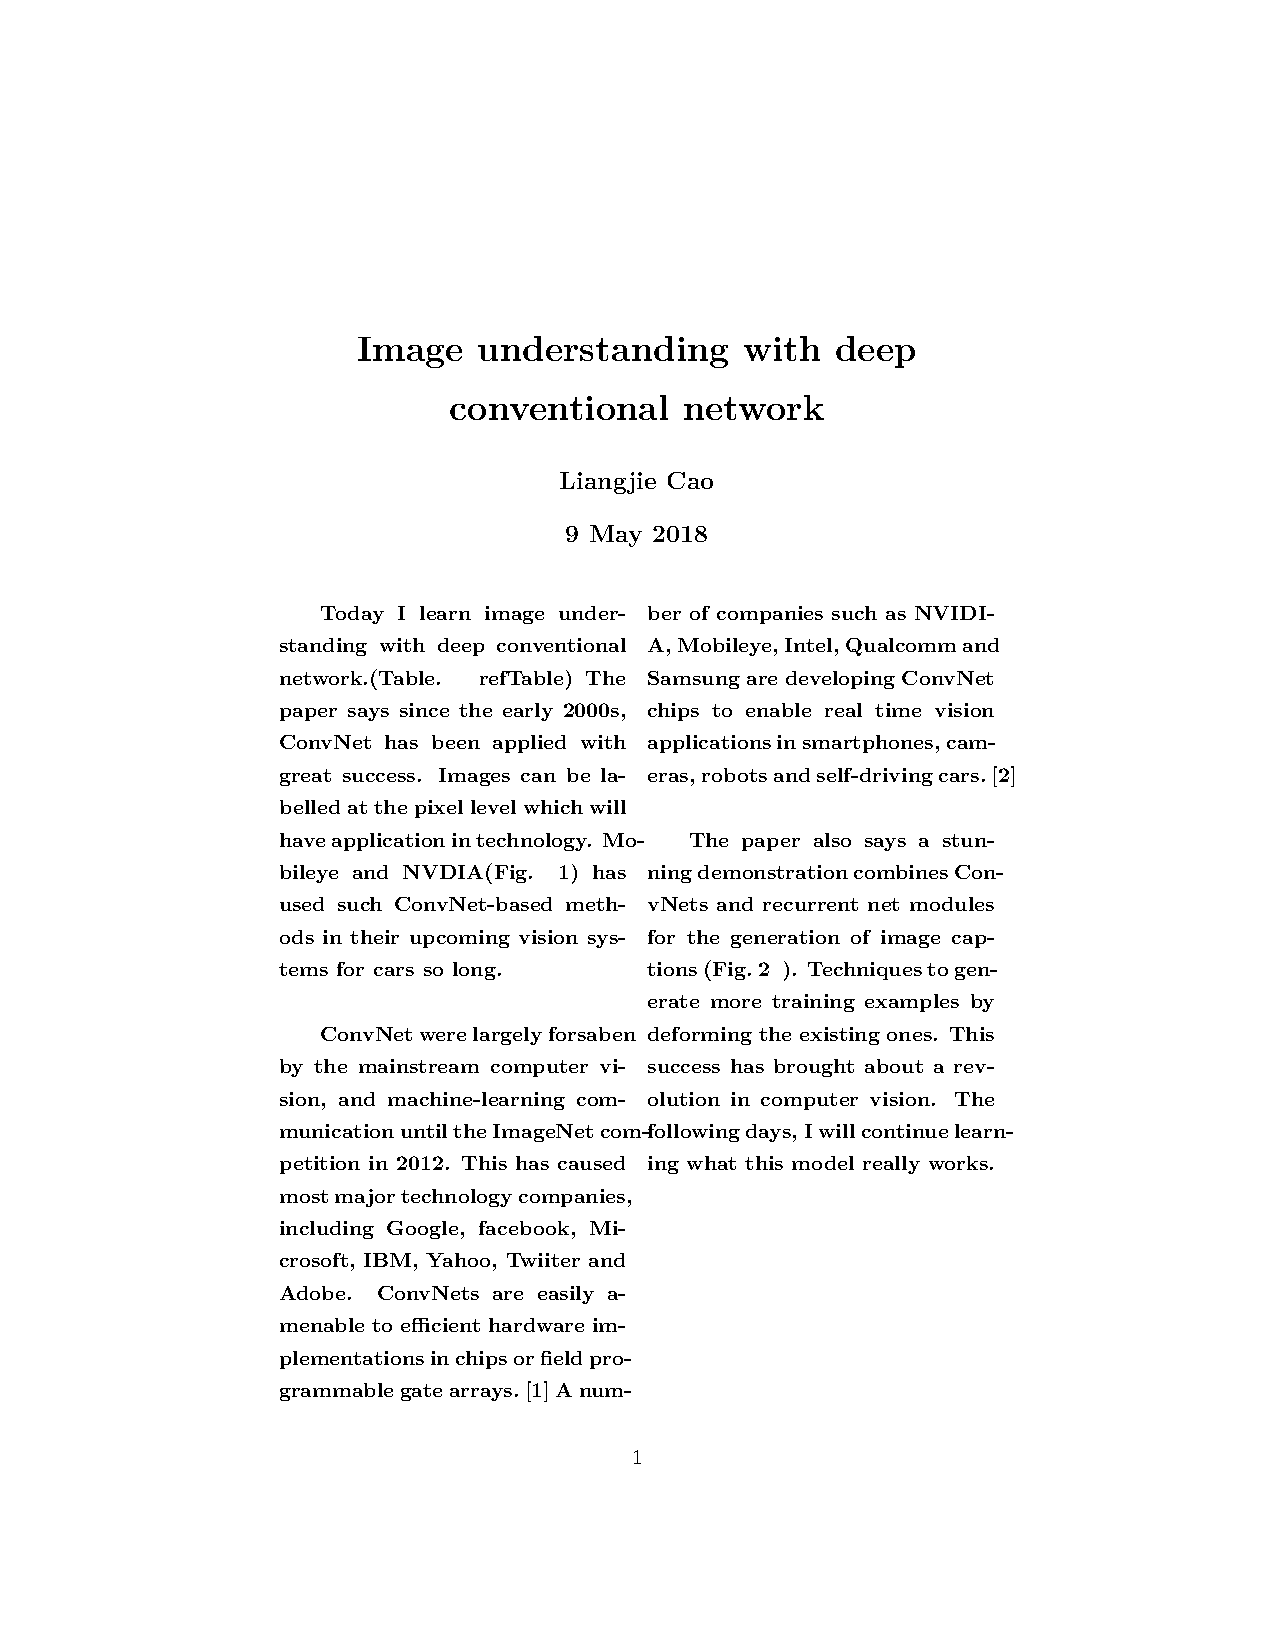
\includegraphics[width=5cm]{image.png}\\
 \caption{\textbf{From image to text}}\label{Figure2}
\end{figure}
\begin{table}[!htbp]
  \centering
 \begin{tabular}{|p{2cm}|p{2cm}|p{2cm}}
   \hline
     1 & convolutional layers\\
  \hline
     2 & pooling layers\\
   \hline
   3 & Relu layer \\
   \hline
  \end{tabular}
  \caption{\textbf{Layers used by ConvNets}} \label{Table}
  \end{table}
\bibliographystyle{plain}
\bibliography{yinyong1,yinyong4}
\end{document}

